% !TEX root = ../main.tex



% FV 2 p.  92
%[2 p. 92] 
\item Van de Empire Stage Building in New York komt op \SI{250}{m} een ijskegel los en valt naar beneden.
\begin{enumerate}
\item Na hoeveel tijd en met welke snelheid bereikt het ijskegeltje uiteindelijk de grond?
\item Hoelang en over welke afstand moet de ijskegel al gevallen zijn om in de daaropvolgende \SI{2}{s} een afstand te kunnen afleggen van \SI{100}{m}?
\end{enumerate}
\begin{oplossing}
\item[Gegeven]$x_3=\SI{250}{m}$\newline$\Delta t=t_2-t_1=\SI{2,0}{s}$\newline$\Delta x=x_2-x_1=\SI{100}{m}$
\item[Gevraagd]$t_3,v_3,t_1$ en $x_1$
\item[Oplossing]
\begin{enumerate}

\item\begin{minipage}[t]{0.63\linewidth}
	Omdat de beweging enkel naar beneden is, is de beschrijving gemakkelijk met een $x$-as naar beneden gericht. De versnellingscomponent $a$ is dan gelijk aan de valversnelling $g$. Omdat de kegel vanuit rust vertrekt, vinden we de valtijd uit $x=\frac{1}{2}gt^2$:
\begin{equation*}
t=\sqrt{\frac{2x}{g}}
\end{equation*}
De valtijd bepaalt de eindsnelheid:
\begin{equation*}
v=gt=g\sqrt{\frac{2x}{g}}=\sqrt{2gx}
\end{equation*}
\end{minipage}%
\begin{minipage}[t]{0.37\linewidth}
	\raisebox{1ex-\height}{%
	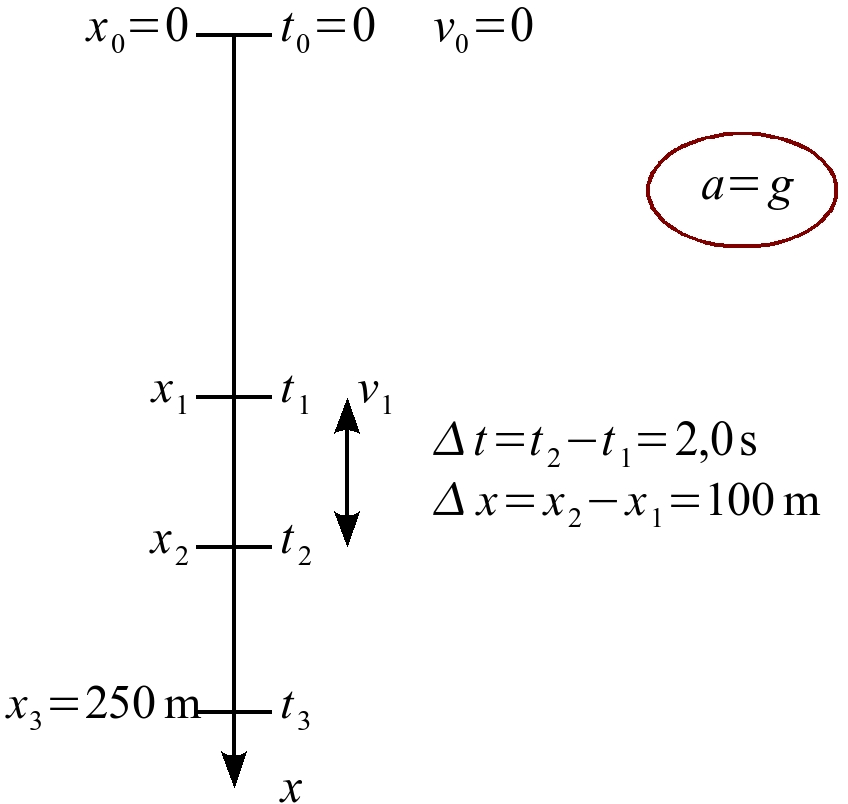
\includegraphics[height=5cm]{opdr16p28}%
	}
\end{minipage}

Invullen van de gegevens geeft $t_3=\SI{7,1}{s}$ en $v_3=\SI{70}{m/s}=\SI{252}{km/h}$.

\item Uit de plaatsfunctie kunnen we de beginsnelheid\footnote{Voor de honderd meter is de beginsnelheid $v_1$.} halen. De beginsnelheid $v_1$ is immers de enige onbekende in de vergelijking:\footnote{Hoe komen we aan deze uitdrukking? De plaatsfunctie toegepast op de honderd meter geeft: $x_2=x_1+v_1t+\frac{1}{2}gt^2$ waarin de variabele $t$ de verstreken tijd tussen tussen de posities $x_1$ en $x_2$ weergeeft. In dit geval stellen we die echter voor door $\Delta t$. Ook is $\Delta x=x_2-x_1$.}
\begin{equation*}
\Delta x=v_1\Delta t+\frac{1}{2}g\Delta t^2\\
\end{equation*}
Dus: $v_1=\frac{2\Delta x-g\Delta t^2}{2\Delta t}$.\footnote{Als we de uitdrukking uitwerken: $v_1=\frac{2\Delta x-g\Delta t^2}{2\Delta t}=\frac{\Delta x}{\Delta t}-g\frac{\Delta t}{2}=\bar{v}-g\frac{\Delta t}{2}$, is te zien dat $v_1$ \'e\'en seconde eerder dan de gemiddelde snelheid bereikt wordt. De gemiddelde snelheid is immers $\bar{v}=\frac{v_1+v_2}{2}$ en wordt dus halverwege de valtijd van de honderd meter bereikt. Bovendien toont deze uitwerking dat we het vraagstuk ook anders hadden kunnen oplossen. Uit $\frac{\Delta x}{\Delta t}=\frac{v_1+v_2}{2}=\frac{v_1+(v_1+g\Delta t)}{2}$ is immers $v_1$ te bepalen.}
%\begin{equation*}
%v_1=\frac{2\Delta x-g\Delta t^2}{2\Delta t}%\\
%%&=&\frac{\Delta x}{\Delta t}-g\frac{\Delta t}{2}\\
%%&=&\bar{v}-g\frac{\Delta t}{2}
%\end{equation*}
%\end{minipage}%
%\begin{figure}[h]
%\centering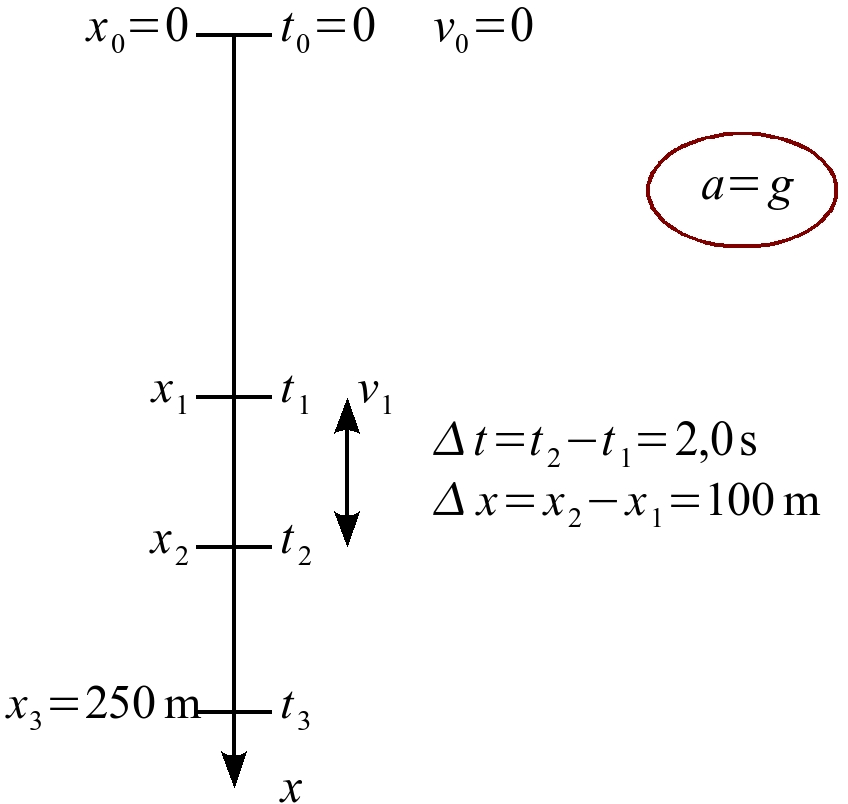
\includegraphics[width=0.4\textwidth]{opdr16p28}
%\end{figure}
Omdat de kegel vanuit rust begint te vallen en per seconde \SI{9,81}{m/s} sneller valt, vinden we de valtijd als $t_1=\frac{v_1}{g}$:
\begin{eqnarray*}
%\Delta x&=&v_1\Delta t+\frac{1}{2}g\Delta t^2\\
%&\Downarrow&(v_1=gt_1)\\
%&=&gt_1\Delta t+\frac{1}{2}g\Delta t^2\\
%&\Updownarrow&\\
t_1=\frac{2\Delta x-g\Delta t^2}{2g\Delta t}&=&\frac{2\cdot100\rm\,m-9,81\rm\,m/s^2\cdot(2,0\rm\,s)^2}{2\cdot9,81\rm\,m/s^2\cdot2,0\rm\,s}=4,1\,s
\end{eqnarray*}
De bijbehorende afgelegde weg is dan $x_1=\frac{1}{2}gt_1^2=82\rm\,m$.
\end{enumerate}
\end{oplossing}